% Venue-agnostic preprint. Compiles with a standard TeX Live / Overleaf install
% (no venue .sty needed). For a camera-ready, swap \documentclass for the venue
% template (USENIX/IEEE/ACM) -- the body uses only standard packages.
\documentclass[10pt,twocolumn]{article}

\usepackage[utf8]{inputenc}
\usepackage[T1]{fontenc}
\usepackage[margin=0.85in]{geometry}
\usepackage{graphicx}
\usepackage{booktabs}
\usepackage{amsmath}
\usepackage{amssymb}
\usepackage{microtype}
\usepackage{xcolor}
\usepackage[hidelinks]{hyperref}
\usepackage{url}

\newcommand{\code}[1]{\texttt{\small #1}}

\title{\textbf{Realisability Belongs in the Search, Not the Filter:\\
A Measurement Pitfall in Adversarial Network-Intrusion-Detection Evaluation}}

\author{Topias Nyg\aa{}rd\\
\small Independent / \emph{(affiliation placeholder)}\\
\small \texttt{github.com/nyymuudi/evasion-arms-race}}

\date{}

\begin{document}
\maketitle

\begin{abstract}
Adversarial evaluation of machine-learning network-intrusion detectors is known
to inflate attacker success when perturbations are measured in feature space
rather than in the space of sendable traffic. The standard remedy is a
\emph{realisability constraint}: keep only the perturbations that correspond to a
packet stream the attacker could actually emit. We show that \emph{how} this
constraint is applied silently decides the result. Applying realisability as a
\emph{post-filter} on a free feature-space search and applying it as a
\emph{constraint on the search itself} give opposite conclusions on the same
detector, with the same feasibility definition and the same attack. On
CIC-IDS2017 DoS-Hulk, a decision-based black-box boundary attack evades a random
forest with $0\%$ realisable success under post-filtering---suggesting robustness
to feasible attacks---but $100\%$ realisable success when the search is confined
to the realisable manifold; logistic regression rises from $45\%$ to $85\%$. The
post-filtered $0\%$ is an artefact: the free search never looked on the manifold,
so the filter declared its off-manifold output impossible. The result is
converged (it does not move with $2.5\times$ the query budget), so it is not a
weak-attacker artefact. We arrived at this through a pre-registered stress test
that overturned our own earlier headline; we report that self-correction as part
of the contribution. We give a concrete manifold projection that makes any
boundary search realisability-constrained by construction, and we trace the
consequences to data poisoning and adversarial training, where the same
measurement choice changes the conclusion. The lesson is methodological:
realisability must shape the search, not be bolted on afterwards, or reported
robustness may be an artefact of where the search was allowed to look. Code,
data-processing, and every figure are reproducible from a single repository.
\end{abstract}

\section{Introduction}

Adversarial examples reliably fool machine-learning classifiers
\cite{szegedy2014intriguing,goodfellow2015explaining}, and network-intrusion
detection systems (NIDS) are no exception. But a NIDS adversary does not perturb a
feature vector; it sends packets. A perturbation is only meaningful if it
corresponds to traffic the attacker can actually emit while preserving the
attack's function. Optimising directly in feature space therefore over-states the
threat: many ``adversarial flows'' map to no packet stream at all. This
\emph{feature-space inflation} is well documented, and the recommended discipline
is to work in the \emph{problem space}---to generate or verify real objects rather
than feature vectors~\cite{pierazzi2020problemspace,apruzzese2022realistic}, in
line with broader warnings about evaluation pitfalls in security
ML~\cite{arp2022dodo}.

We identify a \emph{third}, less-recognised bias that survives even when an author
adopts a realisability constraint: \textbf{the difference between applying
realisability as a post-hoc filter and applying it as a constraint on the search}.
The natural and common implementation searches feature space freely, then keeps
the adversarial examples that pass a feasibility check. We show this
under-reports---and can invert---the conclusion, because a free search wanders
into infeasible regions and the filter then discards results without ever asking
whether feasible evasions exist elsewhere.

Concretely (Section~\ref{sec:three}), on CIC-IDS2017 DoS-Hulk a single
decision-based black-box boundary attack yields, against a random forest:
$\sim$$90\%$ success in feature space, $\mathbf{0\%}$ realisable success under a
post-filter, and $\mathbf{100\%}$ realisable success when the \emph{same} attack
is confined to the realisable manifold. Logistic regression goes $100\%\!\to\!45\%\!\to\!85\%$.
The feasibility \emph{definition} is identical across the three numbers; only the
search space differs. The post-filtered $0\%$---which reads as ``the random forest
resists feasible attacks''---is an artefact.

We did not set out to make this point. An earlier version of this work reported
the post-filtered numbers as evidence that realisability rescues the random
forest. A \emph{pre-registered} stress test, designed to attack exactly that
claim, refuted it. We keep that episode in the paper (Section~\ref{sec:honesty}):
the methodological discipline is demonstrated, not merely asserted.

\paragraph{Contributions.}
\begin{itemize}\itemsep2pt
  \item We isolate \emph{post-filtering} as a distinct measurement bias in
  adversarial NIDS evaluation, separate from feature-space inflation, and show it
  can invert the qualitative conclusion (Section~\ref{sec:three}).
  \item We give a deterministic, idempotent \emph{manifold projection} that makes
  any black-box search realisability-constrained by construction, and show the
  five ``unreconstructable'' CICFlowMeter packet-length aggregates are in fact
  recoverable in closed form ($R^2\!\ge\!0.997$) (Section~\ref{sec:manifold}).
  \item We report a pre-registered self-correction in which the measurement choice
  overturned our own headline, as a model for honest evaluation
  (Section~\ref{sec:honesty}).
  \item We trace the same bias into poisoning and adversarial training, and we
  close a temporal-evaluation gap, finding the headline robust to concept drift
  (Sections~\ref{sec:downstream},~\ref{sec:limitations}). Everything is
  reproducible from one repository.
\end{itemize}

\section{Background and Threat Model}
\label{sec:background}

\paragraph{Dataset and detectors.}
We study CIC-IDS2017~\cite{sharafaldin2018cicids}, Wednesday capture, the binary
problem DoS-Hulk vs.\ BENIGN, with the $78$ CICFlowMeter~\cite{lashkari2017cicflowmeter}
flow features ($\sim$$671$k flows after cleaning). We train two detectors on a
shared standardised feature space: $\ell_2$-regularised \emph{logistic regression}
(a smooth decision surface) and a $200$-tree \emph{random
forest}~\cite{breiman2001randomforests} (piecewise-constant). The contrast in
model geometry is deliberate; tree ensembles have their own evasion/hardening
literature~\cite{kantchelian2016evasion}. Both reach PR-AUC $\ge 0.999$ on a
held-out test set, so accuracy is uninformative and we report PR-AUC throughout.

\paragraph{Threat model.}
The attacker has \emph{black-box} query access to the detector's decision, not its
parameters or gradients---the realistic and harder setting. The evasion search is
a decision-based boundary attack in the spirit of
\cite{brendel2018boundary,chen2020hopskipjump}, querying only the hard label,
rather than a score-based estimator such as NES~\cite{ilyas2018blackbox}; a
hard-label attack run identically against both detectors keeps the comparison
fair on the piecewise-constant forest.

\paragraph{The feasibility constraint.}
Every feature is assigned a \emph{control class} by a header-driven rule
classifier: \emph{controllable} (the attacker's own forward timing, sizing,
padding, flags; $30$ features), \emph{constrained} (forward volume/rate and TCP
parameters, bounded to a legal box with a DoS functional floor; $7$),
\emph{frozen} (backward/server direction, connection-level flag counts, service
port; $\sim$$32$), and \emph{derived} (aggregates recomputed from atomic features;
$\sim$$9$). A \emph{feasibility projection} confines any perturbation to features
the attacker controls, within protocol-legal and functionality-preserving bounds
(a DoS flood must remain a flood). This is the control-class realisation of the
problem-space discipline~\cite{pierazzi2020problemspace,apruzzese2022realistic}.

\section{The Realisable Manifold}
\label{sec:manifold}

The feasibility projection above keeps a perturbation in the attacker's
\emph{control set}, but it does not guarantee the result corresponds to any packet
multiset. CICFlowMeter features are moments of a flow's packets, and arbitrary
moment tuples are not jointly realisable. We define the \emph{realisable manifold}
by the necessary moment-consistency conditions a real forward packet multiset
imposes:
\begin{itemize}\itemsep1pt
  \item ordering and range: $0 \le \min \le \mathrm{mean} \le \max$;
  \item totals: $\text{Total Length} = N \cdot \mathrm{mean}$, and
  $\text{IAT Total} = (N{-}1)\cdot \mathrm{IAT\ mean}$;
  \item the Bhatia--Davis variance bound~\cite{bhatia2000variance}
  $\sigma^2 \le (\max-\mathrm{mean})(\mathrm{mean}-\min)$, which is the tight upper
  bound on the variance of any distribution on $[\min,\max]$ with a given mean
  (and is also \emph{sufficient} for such a distribution to exist);
  \item timing sanity: $\text{IAT max} \le \text{flow duration}$.
\end{itemize}
A free feature-space search routinely violates these---it moves the standard
deviation independently of the min/max/mean, producing moment tuples no packet
sequence can realise.

\paragraph{Recovering the ``unreconstructable'' aggregates.}
Five pooled features (Min/Max/Mean/Std/Variance Packet Length) mix both
directions and were previously treated as unreconstructable from per-direction
CICFlowMeter columns. They are not. Min and Max are exact
($\min(\text{fwd}_{\min},\text{bwd}_{\min})$, etc.); Mean, Std, and Variance
follow from the law of total variance applied to the two directions' marginals,
up to a small systematic CICFlowMeter definitional offset that a data-fit affine
calibration removes ($R^2 \ge 0.997$ on real flows). This closed form is what
makes an on-manifold search possible without per-flow packet capture.

\paragraph{Manifold projection.}
We implement \code{manifold\_project}: the feasibility projection followed by a
deterministic, idempotent clamp-and-recompute that enforces exactly the
constraints above and recomputes the dependent aggregates. Crucially this is
\emph{constraint enforcement by construction}, not nearest-point projection onto a
(non-convex) set, so the manifold's non-convexity does not destabilise it. A
boundary attack that calls \code{manifold\_project} on every candidate searches
\emph{only} the realisable manifold; every point the detector scores already
passes the feasibility check.

\section{Realisability at Three Measurement Levels}
\label{sec:three}

We run one experiment ($20$ DoS-Hulk samples, identical attack, identical
feasibility definition) and read evasion success at three levels:
\textbf{(i) feature-space}---success ignoring feasibility;
\textbf{(ii) post-filter}---feature-space successes that pass \code{is\_feasible};
\textbf{(iii) manifold-constrained}---success of the search confined to the
manifold (every success feasible by construction). Figure~\ref{fig:three} and
Table~\ref{tab:three} report the result.

\begin{figure}[t]
  \centering
  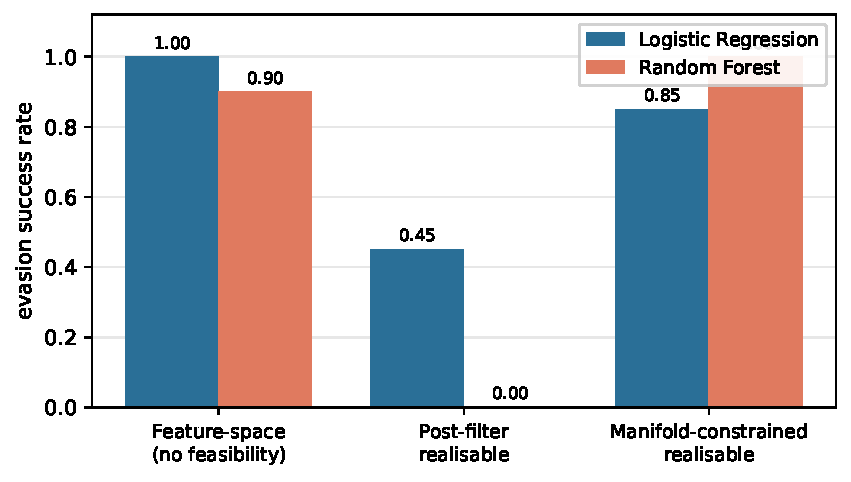
\includegraphics[width=\columnwidth]{figures/three_levels.pdf}
  \caption{Evasion success at three measurement levels (one experiment, one
  feasibility definition; only the search space differs). The random forest
  reads as robust under post-filtering ($0\%$) yet is fully evadable by realisable
  traffic when the search is on the manifold ($100\%$). The $0\%$ is a
  measurement artefact, not robustness.}
  \label{fig:three}
\end{figure}

\begin{table}[t]
  \centering
  \small
  \begin{tabular}{lcc}
    \toprule
    Measurement level & LR & RF \\
    \midrule
    Feature-space (no feasibility) & $1.00$ & $0.90$ \\
    Post-filter realisable & $0.45$ & $\mathbf{0.00}$ \\
    Manifold-constrained realisable & $0.85$ & $\mathbf{1.00}$ \\
    \bottomrule
  \end{tabular}
  \caption{Evasion success rate by measurement level. The post-filter and
  manifold rows use the \emph{same} feasibility definition; they differ only in
  whether realisability constrained the search.}
  \label{tab:three}
\end{table}

The qualitative reading flips with the measurement level. Post-filtering says the
random forest is robust to feasible attacks ($0\%$); the manifold-constrained
search says it is fully evadable ($100\%$). Both use \code{is\_feasible}
identically. The free search produced random-forest evasions that all violated
moment consistency---variance beyond the Bhatia--Davis bound, $\text{IAT max} >
\text{duration}$, $\text{Total} \ne N\cdot\mathrm{mean}$---so the filter zeroed
them, never asking whether feasible evasions existed elsewhere. They do, in
abundance.

\paragraph{It is not a weak-attacker artefact.}
A natural objection is that the manifold search merely needed more power. It did
not: increasing the query budget by $2.5\times$ (to $2000$) and adding restarts
leaves the manifold rates unchanged ($0.85$ / $1.00$), and the manifold
budget--success curve plateaus within $\approx 50$ queries. The two dimensions
are independent: \emph{constraining the search space} addresses the objection,
\emph{adding power} alone would only strengthen it; we vary both. The converged
on-manifold rates are genuine ceilings.

\paragraph{Why the forest, not the line.}
The logistic boundary is linear, so even a manifold-constrained attacker finds
realisable evasions on the far side of a hyperplane ($85\%$); a post-filter still
discards nearly half ($45\%$) because the free search drifts off-manifold. The
forest is piecewise-constant and extrapolates arbitrarily off the training
support; the free search lands in those off-manifold benign regions (which are
infeasible, hence $0\%$ post-filter), while the manifold search finds the forest's
\emph{on-manifold} benign leaves ($100\%$). Post-filtering is maximally
misleading exactly where the model is most irregular.

\section{A Pre-registered Self-Correction}
\label{sec:honesty}

An earlier version of this work reported the post-filter row of
Table~\ref{tab:three} as its headline: feature-space evasion is near-total but
realisable evasion is only $\approx$$45\%$/$0\%$, so realisability ``rescues'' the
random forest. Before publishing we wrote down the obvious objection---a $0\%$ from
post-filtering cannot distinguish robustness from a search that never looked on
the manifold---and pre-registered both outcomes: if a manifold-constrained,
adequately-powered search still yielded $\approx 0\%$, the claim would be upgraded
to evidence; if it rose, the claim was a measurement artefact and would be
withdrawn. It rose to $100\%$. We withdrew the headline.

We keep this episode because it \emph{is} the contribution: the discipline that
distinguishes a credible realisability study from an over-sold one is
demonstrated, not asserted. The instrument that caught the error---a constrained,
powered search used as a falsification test---is the same instrument we recommend
others apply to their own realisability claims.

\section{Downstream Consequences}
\label{sec:downstream}

The measurement choice propagates beyond evasion.

\paragraph{Poisoning.}
We inject budget-limited, feasibility-projected DoS-Hulk flows labelled benign
into the detector's retraining set and evaluate on clean held-out data, in the
classic poisoning setting~\cite{biggio2012poisoning}. Threshold-independent
detection barely moves even at a $20\%$ poison budget (LR PR-AUC
$0.9993\!\to\!0.9968$; RF $1.0000\!\to\!0.9996$): the strong class separability
resists poisoning of the \emph{ranking}. The deployed \emph{operating point} does
degrade---at a $0.5$ threshold, Hulk recall falls to $\approx0.70$ (LR) /
$\approx0.75$ (RF) at $20\%$ label-flip poison. The realistic auto-labelling
attacker, whose injected flows must be \emph{successful realisable evasions} to
enter with a benign label, is gated by exactly the realisable-evasion rate that
the measurement choice decides: under the corrected (manifold) rate that channel
is open, not closed.

\paragraph{Adversarial training.}
Folding the attacker's realisable evasions back into training (the defensive dual
of poisoning) and iterating an attack/retrain loop, adversarial training buys
\emph{limited, detector-dependent, incomplete} robustness when measured on the
manifold: logistic-regression realisable evasion stays at $100\%$ across four
rounds (a linear boundary cannot carve the benign half of the manifold out from
under the attacker), while the random forest drops $97\%\!\to\!\approx30\%$ after
one round but then plateaus and drifts back up, never reaching zero---at
negligible clean cost. The free-search post-filter, by contrast, reports a tidy
``converges to $0\%$'' for logistic regression that the manifold measurement flatly
contradicts: the bias distorts the \emph{defence} conclusion too.

\section{Limitations and Threats to Validity}
\label{sec:limitations}

\paragraph{Temporal evaluation.}
Our detectors use a stratified random split. We additionally evaluate a
\emph{temporal} split on the timestamped GeneratedLabelledFlows distribution,
having (i) dropped collection-artefact metadata (Flow ID, source/destination IP,
source port, protocol; a model must not learn ``this IP $=$ attack''), and (ii)
parsed CIC's day-first, 12-hour, no-AM/PM timestamps explicitly rather than letting
a generic parser silently mis-order them. DoS-Hulk is a single $24$-minute burst,
so a global early/late split is degenerate (zero positives in the test fold); we
cut at the attack's median timestamp. Concept drift is small (PR-AUC: LR
$-0.0031$, RF $-0.0010$ vs.\ stratified), so the headline is not a split artefact.
Dropping the IP/Flow-ID metadata does not dent the baseline, corroborating that
the detector does not ride collection artefacts.

\paragraph{Realisability definition.}
``Realisable'' here means ``passes the moment-consistency check.'' These
conditions are necessary, and Bhatia--Davis is sufficient for a real-valued
multiset; a stricter oracle (a full packet-capture re-extraction through the
CICFlowMeter binary) could lower the absolute rates. It could not rescue the
post-filtered $0\%$: the manifold search already exhibits feasible evasions the
filter declared impossible, which is the paper's point. Strengthening the oracle
is future work.

\paragraph{Scope.}
We study one dataset, one attack class (DoS-Hulk), and two classical detectors,
not deep models. The phenomenon---a search-space versus filter measurement
choice---is general, but its magnitude on other datasets, attacks, and model
families is open. The corrected CIC-IDS2017 extraction
LYCOS-IDS2017~\cite{rosay2021lycos} is a natural next target; our pipeline is
header-driven and switching to it is a header swap.

\section{Conclusion}

Realisability is now standard practice in adversarial NIDS evaluation, but
\emph{how} it is enforced is not standardised, and it decides the result.
Applied as a post-filter on a free feature-space search, realisability
under-reports evasion and can invert the conclusion---most severely for irregular
models like random forests, where it turned $100\%$ realisable evasion into an
apparent $0\%$. Applied as a constraint on the search, it measures what the
attacker can actually do. The fix is simple and cheap: project every candidate
onto the realisable manifold inside the search loop. We recommend that
realisability claims be accompanied by a constrained, powered falsification test,
and we provide one, along with a fully reproducible implementation.

\paragraph{Availability.}
All code, data processing, experiments, and figures are reproducible from
\url{https://github.com/nyymuudi/evasion-arms-race}; each result names the script
that regenerates it.

\bibliographystyle{plain}
\bibliography{references}

\end{document}
